\documentclass{article}

\usepackage{amsmath,graphicx,pslatex}
\usepackage[pdftex,colorlinks]{hyperref}

\begin{document}
\title{This is the SDS 322 \LaTeX{} demo}
\author{Your esteemed professor}
\maketitle

\section{Introduction}
We are going to
add text to this document.
add text to this document.

We are all great programmers, like Margaret Hamilton (see figure~\ref{fig:apollo})
\begin{figure}[ht]
  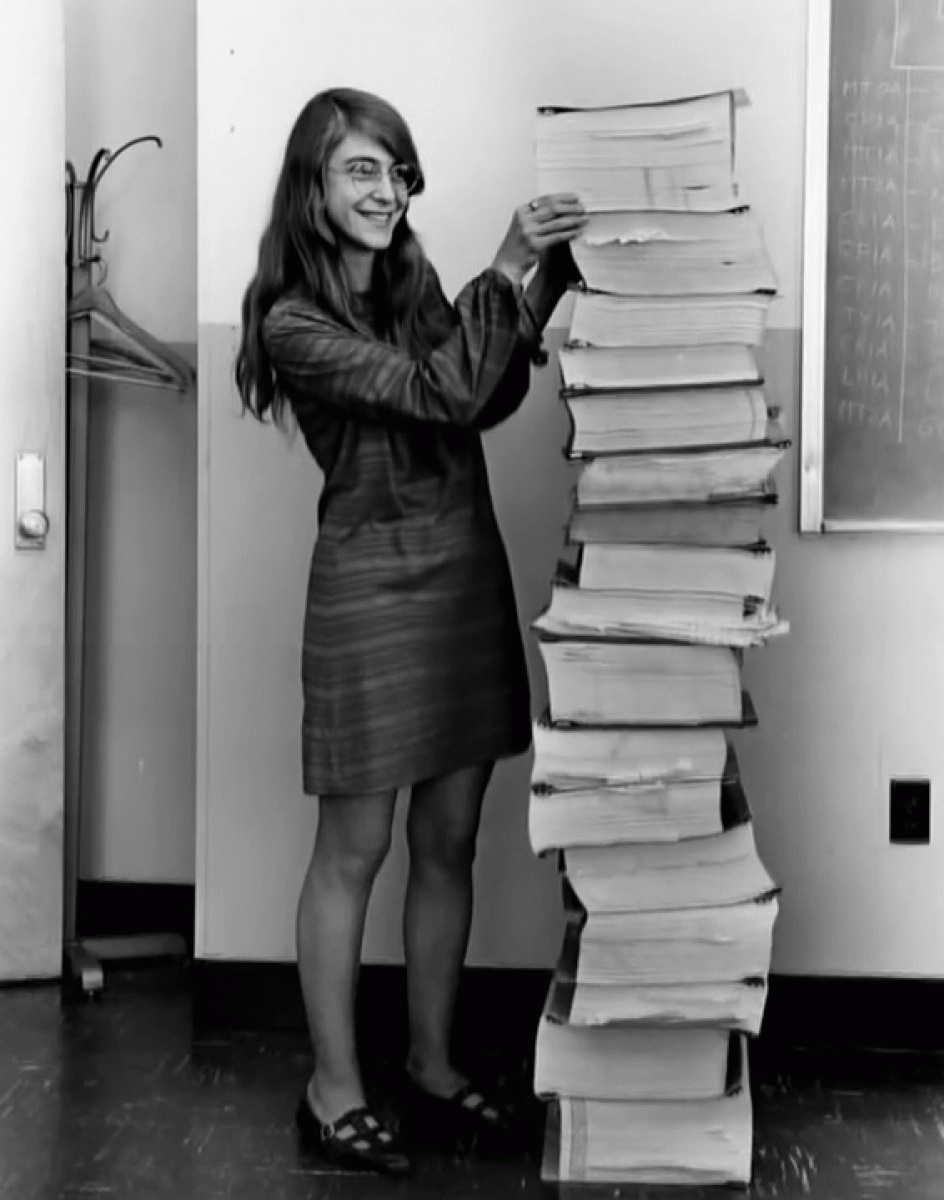
\includegraphics[scale=.1]{hamilton}
  \caption{Margaret Hamilton with homework assignment}
  \label{fig:apollo}
\end{figure}
add text to this document.
add text to this document.
\begin{equation}
  y=
  \begin{cases}
    0&x>0 \\
    1&\text{in all other cases} \\
  \end{cases}
\end{equation}
add text to this document; in particular in section \ref{sec:story}.

A newline $\nu=2\pi$ means a new paragraph. A newline means a new paragraph. A
newline means a new paragraph. $\int_0^1$ A newline means a new paragraph.
\[ x_i^j = \int_i^j xdx \] 
A
newline means a new paragraph.

\section{The whole story}
Here we are going to explain the story.

\subsection{The actual story}
\label{sec:story}

There is stuff here.
For details, see \cite{Eijkhout:hpc}.

\section{Results}

\begin{tabular}{c|l|l}
  \hline
  Names& EID & grades \\
  \hline
  Person 1& asd123 & A \\
  Person 2& sldkfj2897498237 & B- \\
  \hline
\end{tabular}

\bibliography{books}
\bibliographystyle{plain}

\end{document}
